% Source PDF page 141 (printed p. 127)
\section{优化问题}
\subsection{基本术语}
我们用记号
\begin{equation}
\begin{array}{ll}
\text{最小化}&f_0(x)\\
\text{约束为}&f_i(x)\le0,\quad i=1,\ldots,m,\\
&h_i(x)=0,\quad i=1,\ldots,p
\end{array}\tag{4.1}
\end{equation}
表示这样一个问题：在满足条件 $f_i(x)\le0$（$i=1,\ldots,m$）和 $h_i(x)=0$（$i=1,\ldots,p$）的所有 $x$ 中，求使 $f_0(x)$ 最小的 $x$。我们称 $x\in\R^n$ 为优化变量，称函数 $f_0:\R^n\to\R$ 为目标函数或成本函数。不等式 $f_i(x)\le0$ 称为不等式约束，对应的函数 $f_i:\R^n\to\R$ 称为不等式约束函数。等式 $h_i(x)=0$ 称为等式约束，函数 $h_i:\R^n\to\R$ 称为等式约束函数。若没有约束，即 $m=p=0$，就称问题（4.1）为无约束问题。

目标函数和全部约束函数都有定义的点构成的集合
\[
\mathcal D=\bigcap_{i=0}^m\dom f_i\ \cap\ \bigcap_{i=1}^p\dom h_i
\]
称为优化问题（4.1）的定义域。若点 $x\in\mathcal D$ 满足约束 $f_i(x)\le0$（$i=1,\ldots,m$）及 $h_i(x)=0$（$i=1,\ldots,p$），就称它为可行点。若至少存在一个可行点，就称问题（4.1）可行；否则称其不可行。全部可行点构成的集合称为可行集或约束集。

问题（4.1）的最优值 $p^\star$ 定义为
\[
p^\star=\inf\{f_0(x)\mid f_i(x)\le0,\ i=1,\ldots,m,\ h_i(x)=0,\ i=1,\ldots,p\}.
\]
我们允许 $p^\star$ 取广义值 $\pm\infty$。若问题不可行，则 $p^\star=\infty$，这里采用空集下确界为 $\infty$ 的通常约定。

% Source PDF page 142 (printed p. 128)
若存在可行点序列 $x_k$，使 $k\to\infty$ 时 $f_0(x_k)\to-\infty$，则 $p^\star=-\infty$，此时称问题（4.1）无下界。

\subsubsection*{最优点与局部最优点}
若 $x^\star$ 可行且 $f_0(x^\star)=p^\star$，我们就称 $x^\star$ 为最优点，或说它解出了问题（4.1）。全部最优点构成最优集，记为
\[
X_{\mathrm{opt}}=\{x\mid f_i(x)\le0,\ i=1,\ldots,m,\ h_i(x)=0,\ i=1,\ldots,p,\ f_0(x)=p^\star\}.
\]
若问题（4.1）存在最优点，就称最优值能够取到或达到，并称问题可解。若 $X_{\mathrm{opt}}$ 为空，则称最优值不能取到或达到。（问题无下界时总是如此。）满足 $f_0(x)\le p^\star+\epsilon$（其中 $\epsilon>0$）的可行点 $x$ 称为 $\epsilon$ 次优点，全部 $\epsilon$ 次优点构成的集合称为问题（4.1）的 $\epsilon$ 次优集。

若存在 $R>0$，使可行点 $x$ 满足
\[
f_0(x)=\inf\{f_0(z)\mid f_i(z)\le0,\ i=1,\ldots,m,\ h_i(z)=0,\ i=1,\ldots,p,\ \norm{z-x}_2\le R\},
\]
就称 $x$ 为局部最优点。换言之，$x$ 解出了以 $z$ 为变量的优化问题
\[
\begin{array}{ll}
\text{最小化}&f_0(z)\\
\text{约束为}&f_i(z)\le0,\quad i=1,\ldots,m,\\
&h_i(z)=0,\quad i=1,\ldots,p,\\
&\norm{z-x}_2\le R.
\end{array}
\]
粗略地说，这意味着 $x$ 在可行集中邻近的点上使 $f_0$ 最小。有时用“全局最优”代替“最优”，以区别于“局部最优”。不过，本书中的“最优”始终指全局最优。

若 $x$ 可行且 $f_i(x)=0$，就称第 $i$ 个不等式约束 $f_i(x)\le0$ 在 $x$ 处是活跃的。若 $f_i(x)<0$，则称该约束不活跃。（等式约束在所有可行点处都是活跃的。）若删除一个约束不改变可行集，就称它是冗余约束。

\begin{origexample}{4.1}
我们用几个简单的无约束优化问题说明上述定义，其中变量 $x\in\R$，且 $\dom f_0=\R_{++}$。
\begin{itemize}
\item $f_0(x)=1/x$：$p^\star=0$，但最优值不能达到。
\item $f_0(x)=-\log x$：$p^\star=-\infty$，所以问题无下界。
\item $f_0(x)=x\log x$：$p^\star=-1/e$，在唯一最优点 $x^\star=1/e$ 处达到。
\end{itemize}
\end{origexample}

\subsubsection*{可行性问题}
若目标函数恒为零，则最优值或者为零（可行集非空时），或者为 $\infty$（可行集为空时）。我们称其为可行性问题，有时写为

% Source PDF page 143 (printed p. 129)
\[
\begin{array}{ll}
\text{求}&x\\
\text{使得}&f_i(x)\le0,\quad i=1,\ldots,m,\\
&h_i(x)=0,\quad i=1,\ldots,p.
\end{array}
\]
因此，可行性问题就是判断约束是否相容；若相容，则求一个满足全部约束的点。

\subsection{将问题写成标准形式}
我们称（4.1）为标准形式优化问题。在标准形式中，约定不等式和等式约束的右端均为零。将非零右端移到左端，总能做到这一点。例如，把等式约束 $g_i(x)=\widetilde g_i(x)$ 写为 $h_i(x)=0$，其中 $h_i(x)=g_i(x)-\widetilde g_i(x)$。类似地，把 $f_i(x)\ge0$ 写成 $-f_i(x)\le0$。

\begin{origexample}{4.2}
\textbf{盒约束。}考虑优化问题
\[
\begin{array}{ll}
\text{最小化}&f_0(x)\\
\text{约束为}&l_i\le x_i\le u_i,\quad i=1,\ldots,n,
\end{array}
\]
其中变量为 $x\in\R^n$。这些约束称为变量界，因为它们给出每个 $x_i$ 的下界和上界；也称为盒约束，因为可行集是一个盒。

可以将此问题写成标准形式
\[
\begin{array}{ll}
\text{最小化}&f_0(x)\\
\text{约束为}&l_i-x_i\le0,\quad i=1,\ldots,n,\\
&x_i-u_i\le0,\quad i=1,\ldots,n.
\end{array}
\]
共有 $2n$ 个不等式约束函数：
\[
f_i(x)=l_i-x_i,\quad i=1,\ldots,n,
\]
以及
\[
f_i(x)=x_{i-n}-u_{i-n},\quad i=n+1,\ldots,2n.
\]
\end{origexample}

\subsubsection*{最大化问题}
按照惯例，我们主要讨论最小化问题。对于最大化问题
\begin{equation}
\begin{array}{ll}
\text{最大化}&f_0(x)\\
\text{约束为}&f_i(x)\le0,\quad i=1,\ldots,m,\\
&h_i(x)=0,\quad i=1,\ldots,p,
\end{array}\tag{4.2}
\end{equation}

% Source PDF page 144 (printed p. 130)
可在相同约束下最小化函数 $-f_0$ 来求解。利用这一对应关系，可以为最大化问题（4.2）定义上述全部术语。例如，（4.2）的最优值定义为
\[
p^\star=\sup\{f_0(x)\mid f_i(x)\le0,\ i=1,\ldots,m,\ h_i(x)=0,\ i=1,\ldots,p\},
\]
而可行点 $x$ 为 $\epsilon$ 次优点的条件为 $f_0(x)\ge p^\star-\epsilon$。讨论最大化问题时，有时将目标称为效用或满意程度，而非成本。

\subsection{等价问题}
本书以非形式化的方式使用优化问题的等价性概念。如果由一个问题的解容易得到另一个问题的解，反之亦然，就称两个问题等价。（可以严格定义等价性，但定义比较复杂。）

作为一个简单例子，考虑问题
\begin{equation}
\begin{array}{ll}
\text{最小化}&\widetilde f_0(x)=\alpha_0f_0(x)\\
\text{约束为}&\widetilde f_i(x)=\alpha_if_i(x)\le0,\quad i=1,\ldots,m,\\
&\widetilde h_i(x)=\beta_ih_i(x)=0,\quad i=1,\ldots,p,
\end{array}\tag{4.3}
\end{equation}
其中 $\alpha_i>0$（$i=0,\ldots,m$），$\beta_i\ne0$（$i=1,\ldots,p$）。此问题由标准形式问题（4.1）得到：目标函数和不等式约束函数分别乘以正数，等式约束函数分别乘以非零常数。因此，（4.3）与原问题（4.1）的可行集相同。点 $x$ 为原问题（4.1）的最优点，当且仅当它为缩放后问题（4.3）的最优点，所以我们称两个问题等价。但这两个问题并不相同（除非所有 $\alpha_i$ 和 $\beta_i$ 均为一），因为目标函数和约束函数不同。下面介绍几种产生等价问题的一般变换。

\subsubsection*{变量变换}
设 $\phi:\R^n\to\R^n$ 是一一映射，其像包含问题的定义域 $\mathcal D$，即 $\phi(\dom\phi)\supseteq\mathcal D$。定义函数 $\widetilde f_i$ 和 $\widetilde h_i$ 为
\[
\widetilde f_i(z)=f_i(\phi(z)),\quad i=0,\ldots,m,\qquad
\widetilde h_i(z)=h_i(\phi(z)),\quad i=1,\ldots,p.
\]
考虑以 $z$ 为变量的问题
\begin{equation}
\begin{array}{ll}
\text{最小化}&\widetilde f_0(z)\\
\text{约束为}&\widetilde f_i(z)\le0,\quad i=1,\ldots,m,\\
&\widetilde h_i(z)=0,\quad i=1,\ldots,p.
\end{array}\tag{4.4}
\end{equation}
我们称标准形式问题（4.1）与问题（4.4）由变量变换或变量代换 $x=\phi(z)$ 联系起来。两个问题显然等价：若 $x$ 解出问题（4.1），则 $z=\phi^{-1}(x)$ 解出问题（4.4）；若 $z$ 解出问题（4.4），则 $x=\phi(z)$ 解出问题（4.1）。

% Source PDF page 145 (printed p. 131)
\subsubsection*{目标函数和约束函数的变换}
设 $\psi_0:\R\to\R$ 单调递增，$\psi_1,\ldots,\psi_m:\R\to\R$ 满足 $\psi_i(u)\le0$ 当且仅当 $u\le0$，$\psi_{m+1},\ldots,\psi_{m+p}:\R\to\R$ 满足 $\psi_i(u)=0$ 当且仅当 $u=0$。定义复合函数
\[
\widetilde f_i(x)=\psi_i(f_i(x)),\quad i=0,\ldots,m,\qquad
\widetilde h_i(x)=\psi_{m+i}(h_i(x)),\quad i=1,\ldots,p.
\]
相应问题
\[
\begin{array}{ll}
\text{最小化}&\widetilde f_0(x)\\
\text{约束为}&\widetilde f_i(x)\le0,\quad i=1,\ldots,m,\\
&\widetilde h_i(x)=0,\quad i=1,\ldots,p
\end{array}
\]
显然与标准形式问题（4.1）等价；实际上，两者的可行集相同，最优点也相同。（前面将目标函数和约束函数乘以适当常数的例子（4.3），是所有 $\psi_i$ 均为线性函数的特殊情形。）

\begin{origexample}{4.3}
\textbf{最小范数与最小范数平方问题。}考虑以 $x\in\R^n$ 为变量的无约束欧氏范数最小化问题
\begin{equation}
\text{最小化}\quad\norm{Ax-b}_2.\tag{4.5}
\end{equation}
由于范数总是非负，也可以求解
\begin{equation}
\text{最小化}\quad\norm{Ax-b}_2^2=(Ax-b)^\T(Ax-b),\tag{4.6}
\end{equation}
即最小化欧氏范数的平方。问题（4.5）与（4.6）显然等价，最优点相同；但二者并不是同一个问题。例如，（4.5）的目标在任何满足 $Ax-b=0$ 的 $x$ 处都不可微，而（4.6）的目标对所有 $x$ 都可微（实际上是二次函数）。
\end{origexample}

\subsubsection*{松弛变量}
一个简单变换基于这样的观察：$f_i(x)\le0$ 当且仅当存在 $s_i\ge0$，使 $f_i(x)+s_i=0$。利用这一变换，得到问题
\begin{equation}
\begin{array}{ll}
\text{最小化}&f_0(x)\\
\text{约束为}&s_i\ge0,\quad i=1,\ldots,m,\\
&f_i(x)+s_i=0,\quad i=1,\ldots,m,\\
&h_i(x)=0,\quad i=1,\ldots,p,
\end{array}\tag{4.7}
\end{equation}
变量为 $x\in\R^n$ 和 $s\in\R^m$。此问题有 $n+m$ 个变量、$m$ 个不等式约束（$s_i$ 的非负约束）及 $m+p$ 个等式约束。新变量 $s_i$ 称为原不等式约束 $f_i(x)\le0$ 对应的松弛变量。引入松弛变量，就是用一个等式约束和一个非负约束替换每个不等式约束。

问题（4.7）与原标准形式问题（4.1）等价。事实上，若 $(x,s)$ 对问题（4.7）可行，则由于 $s_i=-f_i(x)\ge0$，$x$ 对原问题可行。

% Source PDF page 146 (printed p. 132)
反过来，若 $x$ 对原问题可行，取 $s_i=-f_i(x)$，则 $(x,s)$ 对问题（4.7）可行。类似地，$x$ 为原问题（4.1）的最优点，当且仅当 $(x,s)$ 为问题（4.7）的最优点，其中 $s_i=-f_i(x)$。

\subsubsection*{消去等式约束}
如果能用参数 $z\in\R^k$ 显式表示等式约束
\begin{equation}
h_i(x)=0,\quad i=1,\ldots,p\tag{4.8}
\end{equation}
的全部解，就可以消去问题中的等式约束。具体而言，设函数 $\phi:\R^k\to\R^n$ 满足：$x$ 满足（4.8），当且仅当存在 $z\in\R^k$ 使 $x=\phi(z)$。则优化问题
\[
\begin{array}{ll}
\text{最小化}&\widetilde f_0(z)=f_0(\phi(z))\\
\text{约束为}&\widetilde f_i(z)=f_i(\phi(z))\le0,\quad i=1,\ldots,m
\end{array}
\]
与原问题（4.1）等价。变换后的问题以 $z\in\R^k$ 为变量，有 $m$ 个不等式约束，没有等式约束。若 $z$ 为变换后问题的最优点，则 $x=\phi(z)$ 为原问题的最优点。反过来，若 $x$ 为原问题的最优点，由于它可行，至少存在一个 $z$ 使 $x=\phi(z)$。任何这样的 $z$ 都是变换后问题的最优点。

\subsubsection*{消去线性等式约束}
当全部等式约束均为线性，即形如 $Ax=b$ 时，消元过程可以描述得更明确，在数值上也容易实现。若 $Ax=b$ 不相容，即 $b\notin\mathcal R(A)$，则原问题不可行。假定不是这种情况，记 $x_0$ 为等式约束的任意一个解。取矩阵 $F\in\R^{n\times k}$，满足 $\mathcal R(F)=\mathcal N(A)$，则线性方程 $Ax=b$ 的通解为 $Fz+x_0$，其中 $z\in\R^k$。（可以选取满秩的 $F$，此时 $k=n-\rank A$。）

将 $x=Fz+x_0$ 代入原问题，得到以 $z$ 为变量的问题
\[
\begin{array}{ll}
\text{最小化}&f_0(Fz+x_0)\\
\text{约束为}&f_i(Fz+x_0)\le0,\quad i=1,\ldots,m.
\end{array}
\]
它与原问题等价，没有等式约束，变量数减少了 $\rank A$。

\subsubsection*{引入等式约束}
也可以在问题中引入等式约束和新变量。一般情形描述起来复杂，也不很有启发性，因此我们介绍一个后面会用到的典型例子。考虑问题
\[
\begin{array}{ll}
\text{最小化}&f_0(A_0x+b_0)\\
\text{约束为}&f_i(A_ix+b_i)\le0,\quad i=1,\ldots,m,\\
&h_i(x)=0,\quad i=1,\ldots,p,
\end{array}
\]

% Source PDF page 147 (printed p. 133)
其中 $x\in\R^n$、$A_i\in\R^{k_i\times n}$、$f_i:\R^{k_i}\to\R$。此问题的目标函数和约束函数由函数 $f_i$ 与仿射变换 $A_ix+b_i$ 复合得到。

引入新变量 $y_i\in\R^{k_i}$ 和新等式约束 $y_i=A_ix+b_i$（$i=0,\ldots,m$），构造等价问题
\[
\begin{array}{ll}
\text{最小化}&f_0(y_0)\\
\text{约束为}&f_i(y_i)\le0,\quad i=1,\ldots,m,\\
&y_i=A_ix+b_i,\quad i=0,\ldots,m,\\
&h_i(x)=0,\quad i=1,\ldots,p.
\end{array}
\]
此问题增加了 $k_0+\cdots+k_m$ 个变量，
\[
y_0\in\R^{k_0},\quad\ldots,\quad y_m\in\R^{k_m},
\]
以及 $k_0+\cdots+k_m$ 个等式约束，
\[
y_0=A_0x+b_0,\quad\ldots,\quad y_m=A_mx+b_m.
\]
目标函数与不等式约束彼此独立，即它们涉及不同的优化变量。

\subsubsection*{对部分变量优化}
总有
\[
\inf_{x,y}f(x,y)=\inf_x\widetilde f(x),\qquad\widetilde f(x)=\inf_y f(x,y).
\]
换言之，总可以先对一部分变量最小化，再对剩余变量最小化。这个简单的一般原理可用于把问题变为等价形式。一般情形描述繁琐，也不很有启发性，因此仍用一个例子说明。

设变量 $x\in\R^n$ 分块为 $x=(x_1,x_2)$，其中 $x_1\in\R^{n_1}$、$x_2\in\R^{n_2}$，且 $n_1+n_2=n$。考虑问题
\begin{equation}
\begin{array}{ll}
\text{最小化}&f_0(x_1,x_2)\\
\text{约束为}&f_i(x_1)\le0,\quad i=1,\ldots,m_1,\\
&\widetilde f_i(x_2)\le0,\quad i=1,\ldots,m_2,
\end{array}\tag{4.9}
\end{equation}
其中约束彼此独立，即每个约束函数只依赖于 $x_1$ 或 $x_2$。先对 $x_2$ 最小化，定义 $x_1$ 的函数
\[
\widetilde f_0(x_1)=\inf\{f_0(x_1,z)\mid\widetilde f_i(z)\le0,\ i=1,\ldots,m_2\}.
\]
于是问题（4.9）等价于
\begin{equation}
\begin{array}{ll}
\text{最小化}&\widetilde f_0(x_1)\\
\text{约束为}&f_i(x_1)\le0,\quad i=1,\ldots,m_1.
\end{array}\tag{4.10}
\end{equation}

% Source PDF page 148 (printed p. 134)
\begin{origexample}{4.4}
\textbf{部分变量受约束的二次函数最小化。}考虑一个目标为严格凸二次函数、部分变量无约束的问题：
\[
\begin{array}{ll}
\text{最小化}&x_1^\T P_{11}x_1+2x_1^\T P_{12}x_2+x_2^\T P_{22}x_2\\
\text{约束为}&f_i(x_1)\le0,\quad i=1,\ldots,m,
\end{array}
\]
其中 $P_{11}$ 和 $P_{22}$ 对称。这里可以解析地对 $x_2$ 最小化：
\[
\inf_{x_2}\bigl(x_1^\T P_{11}x_1+2x_1^\T P_{12}x_2+x_2^\T P_{22}x_2\bigr)
=x_1^\T(P_{11}-P_{12}P_{22}^{-1}P_{12}^\T)x_1
\]
（见§A.5.5）。所以原问题等价于
\[
\begin{array}{ll}
\text{最小化}&x_1^\T(P_{11}-P_{12}P_{22}^{-1}P_{12}^\T)x_1\\
\text{约束为}&f_i(x_1)\le0,\quad i=1,\ldots,m.
\end{array}
\]
\end{origexample}

\subsubsection*{上图形式}
标准问题（4.1）的上图形式为
\begin{equation}
\begin{array}{ll}
\text{最小化}&t\\
\text{约束为}&f_0(x)-t\le0,\\
&f_i(x)\le0,\quad i=1,\ldots,m,\\
&h_i(x)=0,\quad i=1,\ldots,p,
\end{array}\tag{4.11}
\end{equation}
变量为 $x\in\R^n$ 和 $t\in\R$。容易看出它与原问题等价：$(x,t)$ 为（4.11）的最优点，当且仅当 $x$ 为（4.1）的最优点且 $t=f_0(x)$。注意，上图形式问题的目标是变量 $x,t$ 的线性函数。

从几何上，上图形式问题（4.11）可以解释为“图空间”$(x,t)$ 中的优化问题：在满足 $x$ 的约束时，在 $f_0$ 的上图中最小化 $t$。图4.1展示了这一点。

\subsubsection*{隐式约束和显式约束}
利用§3.1.2提过的简单技巧，可以重新定义目标函数的定义域，把任何约束隐含在目标中。作为极端情形，标准形式问题可以表示为无约束问题
\begin{equation}
\text{最小化}\quad F(x),\tag{4.12}
\end{equation}
其中 $F$ 定义为 $f_0$，但将其定义域限制在可行集上：
\[
\dom F=\{x\in\dom f_0\mid f_i(x)\le0,\ i=1,\ldots,m,\ h_i(x)=0,\ i=1,\ldots,p\},
\]
对 $x\in\dom F$，令 $F(x)=f_0(x)$。（等价地，可对不可行的 $x$ 定义 $F(x)=\infty$。）问题（4.1）和（4.12）显然等价：两者的可行集、最优点和最优值相同。

当然，这个变换只是一种记号技巧。虽然问题（4.12）至少名义上是无约束的，把约束隐含起来并没有使问题更容易分析或求解。

% Source PDF page 149 (printed p. 135)
\begin{figure}[htbp]
\centering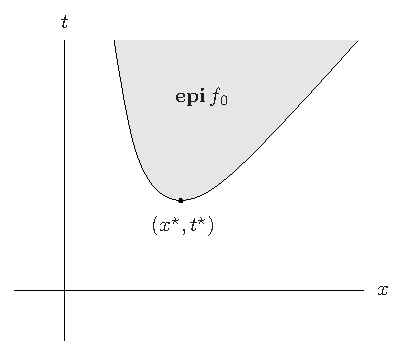
\includegraphics[width=.50\textwidth]{figures/ch04-01.pdf}
\caption*{图4.1\quad 无约束问题的上图形式的几何解释。问题是在上图（阴影部分）中寻找使 $t$ 最小的点，即上图中“最低”的点。最优点为 $(x^\star,t^\star)$。}
\end{figure}
从某些方面说，变换还使问题更困难。例如，假设原问题的目标 $f_0$ 可微，因而其定义域是开集。限制定义域后的目标 $F$ 很可能不可微，因为其定义域很可能不是开集。

反过来，我们也会遇到含有隐式约束的问题，并将其显式化。作为简单例子，考虑无约束问题
\begin{equation}
\text{最小化}\quad f(x),\tag{4.13}
\end{equation}
其中函数 $f$ 为
\[
f(x)=\begin{cases}x^\T x,&Ax=b,\\\infty,&\text{其他情形。}\end{cases}
\]
因此，目标函数在 $Ax=b$ 定义的仿射集上等于二次型 $x^\T x$，在仿射集之外等于 $\infty$。由于显然可以只考虑满足 $Ax=b$ 的点，我们说问题（4.13）的目标中隐藏着一个隐式等式约束 $Ax=b$。可将它显式化，形成等价问题
\begin{equation}
\begin{array}{ll}\text{最小化}&x^\T x\\\text{约束为}&Ax=b.\end{array}\tag{4.14}
\end{equation}
问题（4.13）和（4.14）显然等价，但并不相同。（4.13）无约束，但目标函数不可微；（4.14）有一个等式约束，但目标函数和约束函数均可微。

% Source PDF page 150 (printed p. 136)
\subsection{参数描述与预言机描述}
对于标准形式问题（4.1），还需要说明如何给定目标函数和约束函数。在许多情况下，这些函数有解析表达式或闭式表达式，即由涉及变量 $x$ 和若干参数的公式给出。例如，二次目标函数形如 $f_0(x)=(1/2)x^\T Px+q^\T x+r$。要给定目标函数，只需给出系数（也称问题参数或问题数据）$P\in\mathbf S^n$、$q\in\R^n$ 和 $r\in\R$。我们称其为参数化问题描述，因为要解的具体问题（即问题实例）由目标函数和约束函数表达式中各参数的取值给定。

在另一些情况下，目标函数和约束函数由预言机模型（也称黑箱模型或子程序模型）描述。在预言机模型中，我们不知道 $f$ 的显式表达式，但可以在任意 $x\in\dom f$ 处计算 $f(x)$（通常还包括某些导数）。这称为查询预言机，通常伴随某种成本，例如时间。我们还知道函数的一些先验信息，如凸性和函数值的界。作为具体例子，考虑最小化函数 $f$ 的无约束问题。函数值 $f(x)$ 和梯度 $\nabla f(x)$ 由一个子程序计算。我们可以在任意 $x\in\dom f$ 处调用子程序，但无法访问源代码。以 $x$ 为参数调用后，子程序返回 $f(x)$ 和 $\nabla f(x)$。注意，在预言机模型中，我们从未真正知道函数本身，只知道查询过的点上的函数值（及某些导数）。（另外还知道给定的先验信息，如可微性和凸性。）

实践中，参数描述与预言机描述之间的区别并不那么鲜明。如果给定参数描述，就可以构造一个预言机，在查询时计算所需函数值和导数。第三部分研究的大多数算法都采用预言机模型，但若限定只求解某个特定的参数化问题族，通常可以提高效率。

\section{凸优化}
\subsection{标准形式凸优化问题}
凸优化问题具有如下形式：
\begin{equation}
\begin{array}{ll}
\text{最小化}&f_0(x)\\
\text{约束为}&f_i(x)\le0,\quad i=1,\ldots,m,\\
&a_i^\T x=b_i,\quad i=1,\ldots,p,
\end{array}\tag{4.15}
\end{equation}
其中 $f_0,\ldots,f_m$ 为凸函数。与一般的标准形式问题（4.1）相比，凸问题额外要求以下三点：
